\documentclass{article}
\usepackage{tikz}
\usepackage[margin = 0.5in]{geometry}
\usepackage{verbatim}

\begin{comment}
6
9
\end{comment}

\begin{document}

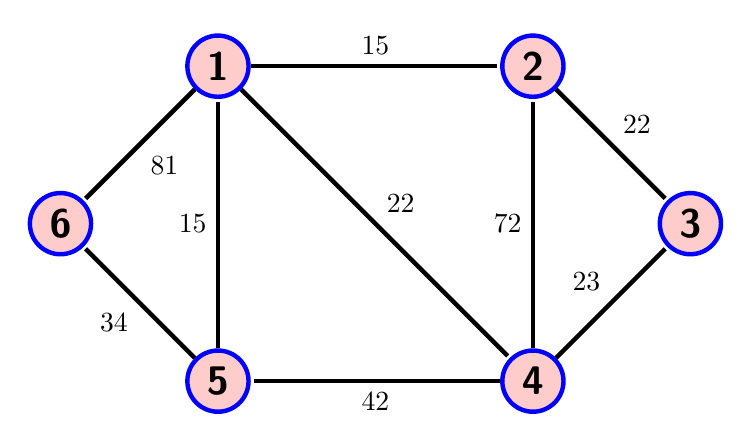
\begin{tikzpicture}[shorten >=1pt, auto, node distance=3cm, ultra thick]

   \begin{scope}[every node/.style={circle,draw=blue,fill=red!20!,font=\sffamily\Large\bfseries}]
    \node (v1) at (-2,2) {1};
    \node (v2) at (2,2) {2};
    \node (v3) at (4,0) {3};
    \node (v4) at (2,-2) {4};
    \node (v5) at (-2,-2) {5};
    \node (v6) at (-4,0) {6};
   \end{scope}
   \begin{scope}[every edge/.style={draw=black,ultra thick}]
   \end{scope}
\draw (v5) edge node{15} (v1);
\draw (v4) edge node{42} (v5);
\draw (v4) edge node{72} (v2);
\draw (v2) edge node{22} (v3);
\draw (v5) edge node{34} (v6);
\draw (v1) edge node{81} (v6);
\draw (v1) edge node{15} (v2);
\draw (v4) edge node{23} (v3);
\draw (v1) edge node{22} (v4);
\end{tikzpicture}

\end{document}
